% Options for packages loaded elsewhere
\PassOptionsToPackage{unicode}{hyperref}
\PassOptionsToPackage{hyphens}{url}
%
\documentclass[
]{article}
\usepackage{amsmath,amssymb}
\usepackage{iftex}
\ifPDFTeX
  \usepackage[T1]{fontenc}
  \usepackage[utf8]{inputenc}
  \usepackage{textcomp} % provide euro and other symbols
\else % if luatex or xetex
  \usepackage{unicode-math} % this also loads fontspec
  \defaultfontfeatures{Scale=MatchLowercase}
  \defaultfontfeatures[\rmfamily]{Ligatures=TeX,Scale=1}
\fi
\usepackage{lmodern}
\ifPDFTeX\else
  % xetex/luatex font selection
\fi
% Use upquote if available, for straight quotes in verbatim environments
\IfFileExists{upquote.sty}{\usepackage{upquote}}{}
\IfFileExists{microtype.sty}{% use microtype if available
  \usepackage[]{microtype}
  \UseMicrotypeSet[protrusion]{basicmath} % disable protrusion for tt fonts
}{}
\makeatletter
\@ifundefined{KOMAClassName}{% if non-KOMA class
  \IfFileExists{parskip.sty}{%
    \usepackage{parskip}
  }{% else
    \setlength{\parindent}{0pt}
    \setlength{\parskip}{6pt plus 2pt minus 1pt}}
}{% if KOMA class
  \KOMAoptions{parskip=half}}
\makeatother
\usepackage{xcolor}
\usepackage[margin=1in]{geometry}
\usepackage{color}
\usepackage{fancyvrb}
\newcommand{\VerbBar}{|}
\newcommand{\VERB}{\Verb[commandchars=\\\{\}]}
\DefineVerbatimEnvironment{Highlighting}{Verbatim}{commandchars=\\\{\}}
% Add ',fontsize=\small' for more characters per line
\usepackage{framed}
\definecolor{shadecolor}{RGB}{248,248,248}
\newenvironment{Shaded}{\begin{snugshade}}{\end{snugshade}}
\newcommand{\AlertTok}[1]{\textcolor[rgb]{0.94,0.16,0.16}{#1}}
\newcommand{\AnnotationTok}[1]{\textcolor[rgb]{0.56,0.35,0.01}{\textbf{\textit{#1}}}}
\newcommand{\AttributeTok}[1]{\textcolor[rgb]{0.13,0.29,0.53}{#1}}
\newcommand{\BaseNTok}[1]{\textcolor[rgb]{0.00,0.00,0.81}{#1}}
\newcommand{\BuiltInTok}[1]{#1}
\newcommand{\CharTok}[1]{\textcolor[rgb]{0.31,0.60,0.02}{#1}}
\newcommand{\CommentTok}[1]{\textcolor[rgb]{0.56,0.35,0.01}{\textit{#1}}}
\newcommand{\CommentVarTok}[1]{\textcolor[rgb]{0.56,0.35,0.01}{\textbf{\textit{#1}}}}
\newcommand{\ConstantTok}[1]{\textcolor[rgb]{0.56,0.35,0.01}{#1}}
\newcommand{\ControlFlowTok}[1]{\textcolor[rgb]{0.13,0.29,0.53}{\textbf{#1}}}
\newcommand{\DataTypeTok}[1]{\textcolor[rgb]{0.13,0.29,0.53}{#1}}
\newcommand{\DecValTok}[1]{\textcolor[rgb]{0.00,0.00,0.81}{#1}}
\newcommand{\DocumentationTok}[1]{\textcolor[rgb]{0.56,0.35,0.01}{\textbf{\textit{#1}}}}
\newcommand{\ErrorTok}[1]{\textcolor[rgb]{0.64,0.00,0.00}{\textbf{#1}}}
\newcommand{\ExtensionTok}[1]{#1}
\newcommand{\FloatTok}[1]{\textcolor[rgb]{0.00,0.00,0.81}{#1}}
\newcommand{\FunctionTok}[1]{\textcolor[rgb]{0.13,0.29,0.53}{\textbf{#1}}}
\newcommand{\ImportTok}[1]{#1}
\newcommand{\InformationTok}[1]{\textcolor[rgb]{0.56,0.35,0.01}{\textbf{\textit{#1}}}}
\newcommand{\KeywordTok}[1]{\textcolor[rgb]{0.13,0.29,0.53}{\textbf{#1}}}
\newcommand{\NormalTok}[1]{#1}
\newcommand{\OperatorTok}[1]{\textcolor[rgb]{0.81,0.36,0.00}{\textbf{#1}}}
\newcommand{\OtherTok}[1]{\textcolor[rgb]{0.56,0.35,0.01}{#1}}
\newcommand{\PreprocessorTok}[1]{\textcolor[rgb]{0.56,0.35,0.01}{\textit{#1}}}
\newcommand{\RegionMarkerTok}[1]{#1}
\newcommand{\SpecialCharTok}[1]{\textcolor[rgb]{0.81,0.36,0.00}{\textbf{#1}}}
\newcommand{\SpecialStringTok}[1]{\textcolor[rgb]{0.31,0.60,0.02}{#1}}
\newcommand{\StringTok}[1]{\textcolor[rgb]{0.31,0.60,0.02}{#1}}
\newcommand{\VariableTok}[1]{\textcolor[rgb]{0.00,0.00,0.00}{#1}}
\newcommand{\VerbatimStringTok}[1]{\textcolor[rgb]{0.31,0.60,0.02}{#1}}
\newcommand{\WarningTok}[1]{\textcolor[rgb]{0.56,0.35,0.01}{\textbf{\textit{#1}}}}
\usepackage{graphicx}
\makeatletter
\def\maxwidth{\ifdim\Gin@nat@width>\linewidth\linewidth\else\Gin@nat@width\fi}
\def\maxheight{\ifdim\Gin@nat@height>\textheight\textheight\else\Gin@nat@height\fi}
\makeatother
% Scale images if necessary, so that they will not overflow the page
% margins by default, and it is still possible to overwrite the defaults
% using explicit options in \includegraphics[width, height, ...]{}
\setkeys{Gin}{width=\maxwidth,height=\maxheight,keepaspectratio}
% Set default figure placement to htbp
\makeatletter
\def\fps@figure{htbp}
\makeatother
\setlength{\emergencystretch}{3em} % prevent overfull lines
\providecommand{\tightlist}{%
  \setlength{\itemsep}{0pt}\setlength{\parskip}{0pt}}
\setcounter{secnumdepth}{-\maxdimen} % remove section numbering
\ifLuaTeX
  \usepackage{selnolig}  % disable illegal ligatures
\fi
\usepackage{bookmark}
\IfFileExists{xurl.sty}{\usepackage{xurl}}{} % add URL line breaks if available
\urlstyle{same}
\hypersetup{
  pdftitle={DS311 - R Lab Assignment},
  pdfauthor={Leslie Contreras},
  hidelinks,
  pdfcreator={LaTeX via pandoc}}

\title{DS311 - R Lab Assignment}
\author{Leslie Contreras}
\date{2024-11-18}

\begin{document}
\maketitle

\subsection{R Assignment 1}\label{r-assignment-1}

\begin{itemize}
\tightlist
\item
  In this assignment, we are going to apply some of the build in data
  set in R for descriptive statistics analysis.
\item
  To earn full grade in this assignment, students need to complete the
  coding tasks for each question to get the result.
\item
  After finished all the questions, knit the document into HTML format
  for submission.
\end{itemize}

\subsubsection{Question 1}\label{question-1}

Using the \textbf{mtcars} data set in R, please answer the following
questions.

\begin{Shaded}
\begin{Highlighting}[]
\CommentTok{\# Loading the data}
\FunctionTok{data}\NormalTok{(mtcars)}

\CommentTok{\# Head of the data set}
\FunctionTok{head}\NormalTok{(mtcars)}
\end{Highlighting}
\end{Shaded}

\begin{verbatim}
##                    mpg cyl disp  hp drat    wt  qsec vs am gear carb
## Mazda RX4         21.0   6  160 110 3.90 2.620 16.46  0  1    4    4
## Mazda RX4 Wag     21.0   6  160 110 3.90 2.875 17.02  0  1    4    4
## Datsun 710        22.8   4  108  93 3.85 2.320 18.61  1  1    4    1
## Hornet 4 Drive    21.4   6  258 110 3.08 3.215 19.44  1  0    3    1
## Hornet Sportabout 18.7   8  360 175 3.15 3.440 17.02  0  0    3    2
## Valiant           18.1   6  225 105 2.76 3.460 20.22  1  0    3    1
\end{verbatim}

\begin{enumerate}
\def\labelenumi{\alph{enumi}.}
\tightlist
\item
  Report the number of variables and observations in the data set.
\end{enumerate}

\begin{Shaded}
\begin{Highlighting}[]
\CommentTok{\# Enter your code here!}
\NormalTok{num\_vars }\OtherTok{\textless{}{-}} \FunctionTok{ncol}\NormalTok{(mtcars)}
\NormalTok{num\_obs }\OtherTok{\textless{}{-}} \FunctionTok{nrow}\NormalTok{(mtcars)}

\CommentTok{\# Answer:}
\FunctionTok{print}\NormalTok{(}\FunctionTok{paste}\NormalTok{(}\StringTok{"There are a total of"}\NormalTok{, num\_vars, }\StringTok{"variables and"}\NormalTok{, num\_obs, }\StringTok{"observations in this dataset."}\NormalTok{))}
\end{Highlighting}
\end{Shaded}

\begin{verbatim}
## [1] "There are a total of 11 variables and 32 observations in this dataset."
\end{verbatim}

\begin{enumerate}
\def\labelenumi{\alph{enumi}.}
\setcounter{enumi}{1}
\tightlist
\item
  Print the summary statistics of the data set and report how many
  discrete and continuous variables are in the data set.
\end{enumerate}

\begin{Shaded}
\begin{Highlighting}[]
\CommentTok{\# Enter your code here!}

\FunctionTok{summary}\NormalTok{(mtcars)}
\end{Highlighting}
\end{Shaded}

\begin{verbatim}
##       mpg             cyl             disp             hp       
##  Min.   :10.40   Min.   :4.000   Min.   : 71.1   Min.   : 52.0  
##  1st Qu.:15.43   1st Qu.:4.000   1st Qu.:120.8   1st Qu.: 96.5  
##  Median :19.20   Median :6.000   Median :196.3   Median :123.0  
##  Mean   :20.09   Mean   :6.188   Mean   :230.7   Mean   :146.7  
##  3rd Qu.:22.80   3rd Qu.:8.000   3rd Qu.:326.0   3rd Qu.:180.0  
##  Max.   :33.90   Max.   :8.000   Max.   :472.0   Max.   :335.0  
##       drat             wt             qsec             vs        
##  Min.   :2.760   Min.   :1.513   Min.   :14.50   Min.   :0.0000  
##  1st Qu.:3.080   1st Qu.:2.581   1st Qu.:16.89   1st Qu.:0.0000  
##  Median :3.695   Median :3.325   Median :17.71   Median :0.0000  
##  Mean   :3.597   Mean   :3.217   Mean   :17.85   Mean   :0.4375  
##  3rd Qu.:3.920   3rd Qu.:3.610   3rd Qu.:18.90   3rd Qu.:1.0000  
##  Max.   :4.930   Max.   :5.424   Max.   :22.90   Max.   :1.0000  
##        am              gear            carb      
##  Min.   :0.0000   Min.   :3.000   Min.   :1.000  
##  1st Qu.:0.0000   1st Qu.:3.000   1st Qu.:2.000  
##  Median :0.0000   Median :4.000   Median :2.000  
##  Mean   :0.4062   Mean   :3.688   Mean   :2.812  
##  3rd Qu.:1.0000   3rd Qu.:4.000   3rd Qu.:4.000  
##  Max.   :1.0000   Max.   :5.000   Max.   :8.000
\end{verbatim}

\begin{Shaded}
\begin{Highlighting}[]
\CommentTok{\# Answer:}
\FunctionTok{print}\NormalTok{(}\StringTok{"There are \_\_3\_\_\_ discrete variables and \_\_\_8\_\_ continuous variables in this data set."}\NormalTok{)}
\end{Highlighting}
\end{Shaded}

\begin{verbatim}
## [1] "There are __3___ discrete variables and ___8__ continuous variables in this data set."
\end{verbatim}

\begin{enumerate}
\def\labelenumi{\alph{enumi}.}
\setcounter{enumi}{2}
\tightlist
\item
  Calculate the mean, variance, and standard deviation for the variable
  \textbf{mpg} and assign them into variable names m, v, and s. Report
  the results in the print statement.
\end{enumerate}

\begin{Shaded}
\begin{Highlighting}[]
\CommentTok{\# Enter your code here!}
\NormalTok{m }\OtherTok{\textless{}{-}} \FunctionTok{mean}\NormalTok{(mtcars}\SpecialCharTok{$}\NormalTok{mpg)}
\NormalTok{v }\OtherTok{\textless{}{-}} \FunctionTok{var}\NormalTok{(mtcars}\SpecialCharTok{$}\NormalTok{mpg)}
\NormalTok{s }\OtherTok{\textless{}{-}} \FunctionTok{sd}\NormalTok{(mtcars}\SpecialCharTok{$}\NormalTok{mpg)}


\FunctionTok{print}\NormalTok{(}\FunctionTok{paste}\NormalTok{(}\StringTok{"The average of miles per gallon (mpg) in this dataset is"}\NormalTok{, }\FunctionTok{round}\NormalTok{(m, }\DecValTok{2}\NormalTok{), }\StringTok{"with variance"}\NormalTok{, }\FunctionTok{round}\NormalTok{(v, }\DecValTok{2}\NormalTok{), }\StringTok{"and standard deviation"}\NormalTok{, }\FunctionTok{round}\NormalTok{(s, }\DecValTok{2}\NormalTok{), }\StringTok{"."}\NormalTok{))}
\end{Highlighting}
\end{Shaded}

\begin{verbatim}
## [1] "The average of miles per gallon (mpg) in this dataset is 20.09 with variance 36.32 and standard deviation 6.03 ."
\end{verbatim}

\begin{Shaded}
\begin{Highlighting}[]
\CommentTok{\# print(paste("The average of Mile Per Gallon from this data set is ",  , " with variance ",  , " and standard deviation",  , "."))}
\end{Highlighting}
\end{Shaded}

\begin{enumerate}
\def\labelenumi{\alph{enumi}.}
\setcounter{enumi}{3}
\tightlist
\item
  Create two tables to summarize 1) average mpg for each cylinder class
  and 2) the standard deviation of mpg for each gear class.
\end{enumerate}

\begin{Shaded}
\begin{Highlighting}[]
\CommentTok{\# Enter your code here!}
\NormalTok{avg\_mpg\_cyl }\OtherTok{\textless{}{-}} \FunctionTok{aggregate}\NormalTok{(mpg }\SpecialCharTok{\textasciitilde{}}\NormalTok{ cyl, }\AttributeTok{data =}\NormalTok{ mtcars, }\AttributeTok{FUN =}\NormalTok{ mean)}
\NormalTok{sd\_mpg\_gear }\OtherTok{\textless{}{-}} \FunctionTok{aggregate}\NormalTok{(mpg }\SpecialCharTok{\textasciitilde{}}\NormalTok{ gear, }\AttributeTok{data =}\NormalTok{ mtcars, }\AttributeTok{FUN =}\NormalTok{ sd)}
\NormalTok{avg\_mpg\_cyl}
\end{Highlighting}
\end{Shaded}

\begin{verbatim}
##   cyl      mpg
## 1   4 26.66364
## 2   6 19.74286
## 3   8 15.10000
\end{verbatim}

\begin{Shaded}
\begin{Highlighting}[]
\NormalTok{sd\_mpg\_gear}
\end{Highlighting}
\end{Shaded}

\begin{verbatim}
##   gear      mpg
## 1    3 3.371618
## 2    4 5.276764
## 3    5 6.658979
\end{verbatim}

\begin{enumerate}
\def\labelenumi{\alph{enumi}.}
\setcounter{enumi}{4}
\tightlist
\item
  Create a crosstab that shows the number of observations belong to each
  cylinder and gear class combinations. The table should show how many
  observations given the car has 4 cylinders with 3 gears, 4 cylinders
  with 4 gears, etc. Report which combination is recorded in this data
  set and how many observations for this type of car.
\end{enumerate}

\begin{Shaded}
\begin{Highlighting}[]
\CommentTok{\# Enter your code here!}
\NormalTok{crosstab }\OtherTok{\textless{}{-}} \FunctionTok{table}\NormalTok{(mtcars}\SpecialCharTok{$}\NormalTok{cyl, mtcars}\SpecialCharTok{$}\NormalTok{gear)}
\NormalTok{crosstab}
\end{Highlighting}
\end{Shaded}

\begin{verbatim}
##    
##      3  4  5
##   4  1  8  2
##   6  2  4  1
##   8 12  0  2
\end{verbatim}

\begin{Shaded}
\begin{Highlighting}[]
\NormalTok{most\_common }\OtherTok{\textless{}{-}} \FunctionTok{which.max}\NormalTok{(crosstab)}
\NormalTok{comb }\OtherTok{\textless{}{-}} \FunctionTok{which}\NormalTok{(crosstab }\SpecialCharTok{==}\NormalTok{ most\_common, }\AttributeTok{arr.ind =} \ConstantTok{TRUE}\NormalTok{)}
\NormalTok{cyl\_class }\OtherTok{\textless{}{-}} \FunctionTok{rownames}\NormalTok{(crosstab)[comb[}\DecValTok{1}\NormalTok{]]}
\NormalTok{gear\_class }\OtherTok{\textless{}{-}} \FunctionTok{colnames}\NormalTok{(crosstab)[comb[}\DecValTok{2}\NormalTok{]]}

\FunctionTok{print}\NormalTok{(}\StringTok{"The most common car type in this data set is car with \_\_\_\_ cylinders and \_\_\_\_ gears. There are total of \_\_\_\_\_ cars belong to this specification in the data set."}\NormalTok{)}
\end{Highlighting}
\end{Shaded}

\begin{verbatim}
## [1] "The most common car type in this data set is car with ____ cylinders and ____ gears. There are total of _____ cars belong to this specification in the data set."
\end{verbatim}

\begin{center}\rule{0.5\linewidth}{0.5pt}\end{center}

\subsubsection{Question 2}\label{question-2}

Use different visualization tools to summarize the data sets in this
question.

\begin{enumerate}
\def\labelenumi{\alph{enumi}.}
\tightlist
\item
  Using the \textbf{PlantGrowth} data set, visualize and compare the
  weight of the plant in the three separated group. Give labels to the
  title, x-axis, and y-axis on the graph. Write a paragraph to summarize
  your findings.
\end{enumerate}

\begin{Shaded}
\begin{Highlighting}[]
\CommentTok{\# Load the data set}
\FunctionTok{data}\NormalTok{(}\StringTok{"PlantGrowth"}\NormalTok{)}

\CommentTok{\# Head of the data set}
\FunctionTok{head}\NormalTok{(PlantGrowth)}
\end{Highlighting}
\end{Shaded}

\begin{verbatim}
##   weight group
## 1   4.17  ctrl
## 2   5.58  ctrl
## 3   5.18  ctrl
## 4   6.11  ctrl
## 5   4.50  ctrl
## 6   4.61  ctrl
\end{verbatim}

\begin{Shaded}
\begin{Highlighting}[]
\CommentTok{\# Enter your code here!}

\FunctionTok{ggplot}\NormalTok{(PlantGrowth, }\FunctionTok{aes}\NormalTok{(}\AttributeTok{x =}\NormalTok{ group, }\AttributeTok{y =}\NormalTok{ weight)) }\SpecialCharTok{+}
  \FunctionTok{geom\_boxplot}\NormalTok{() }\SpecialCharTok{+}
  \FunctionTok{labs}\NormalTok{(}\AttributeTok{title =} \StringTok{"Comparison of Plant Weight by Group"}\NormalTok{, }
       \AttributeTok{x =} \StringTok{"Group"}\NormalTok{, }
       \AttributeTok{y =} \StringTok{"Weight"}\NormalTok{) }\SpecialCharTok{+}
  \FunctionTok{theme\_minimal}\NormalTok{()}
\end{Highlighting}
\end{Shaded}

\includegraphics{RLabLab_files/figure-latex/unnamed-chunk-7-1.pdf}

Result:

=\textgreater{} Report a paragraph to summarize your findings from the
plot!

\begin{enumerate}
\def\labelenumi{\alph{enumi}.}
\setcounter{enumi}{1}
\tightlist
\item
  Using the \textbf{mtcars} data set, plot the histogram for the column
  \textbf{mpg} with 10 breaks. Give labels to the title, x-axis, and
  y-axis on the graph. Report the most observed mpg class from the data
  set.
\end{enumerate}

\begin{Shaded}
\begin{Highlighting}[]
\FunctionTok{hist}\NormalTok{(mtcars}\SpecialCharTok{$}\NormalTok{mpg, }\AttributeTok{breaks =} \DecValTok{10}\NormalTok{, }\AttributeTok{main =} \StringTok{"Histogram of Miles per Gallon (mpg)"}\NormalTok{, }\AttributeTok{xlab =} \StringTok{"Miles per Gallon"}\NormalTok{, }\AttributeTok{ylab =} \StringTok{"Frequency"}\NormalTok{)}
\end{Highlighting}
\end{Shaded}

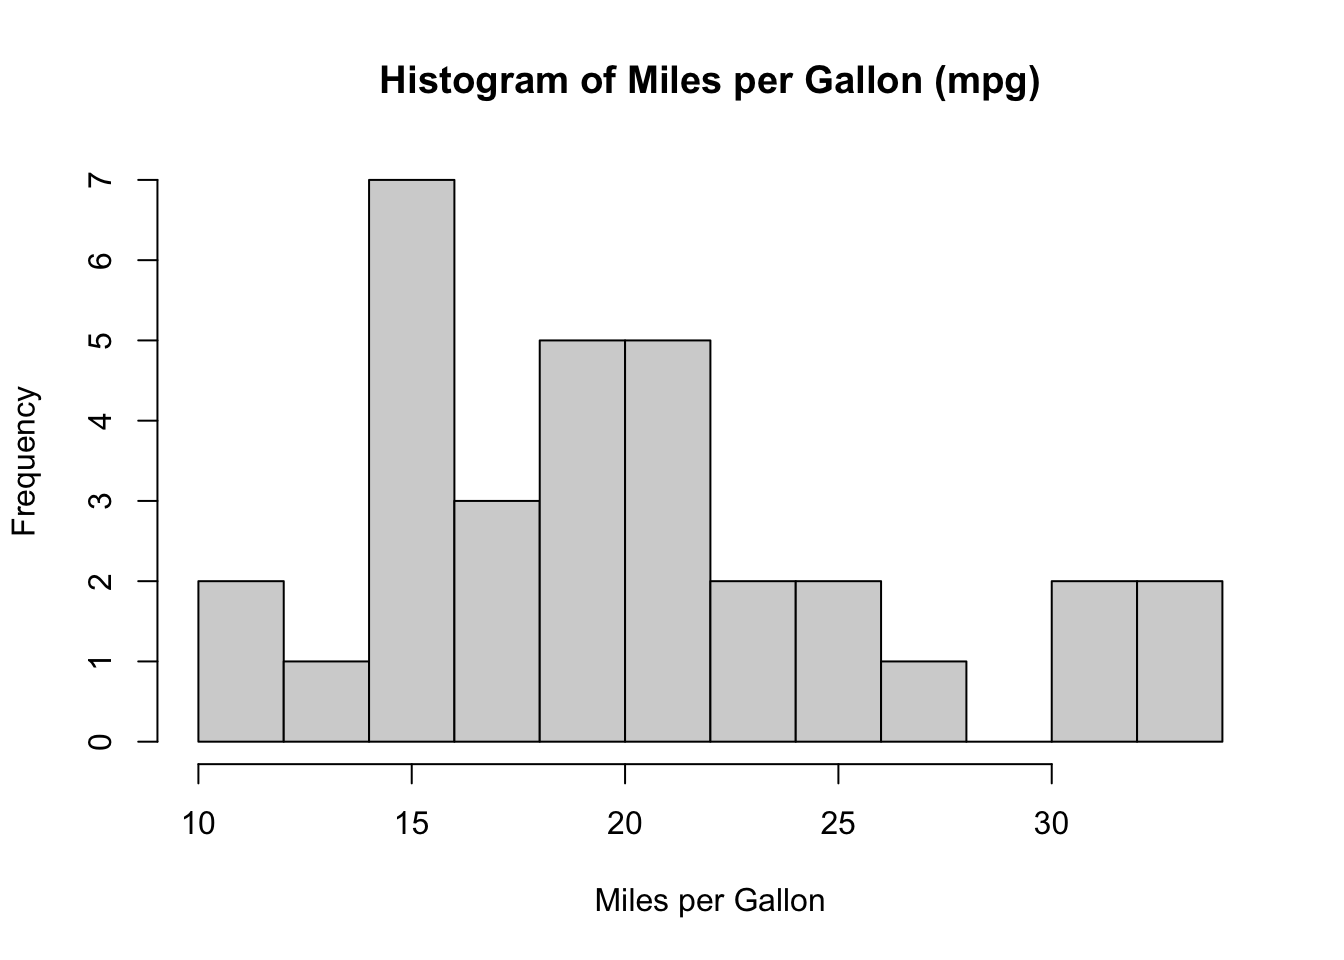
\includegraphics{RLabLab_files/figure-latex/unnamed-chunk-8-1.pdf}

\begin{Shaded}
\begin{Highlighting}[]
\NormalTok{most\_common\_mpg }\OtherTok{\textless{}{-}} \FunctionTok{which.max}\NormalTok{(}\FunctionTok{table}\NormalTok{(}\FunctionTok{cut}\NormalTok{(mtcars}\SpecialCharTok{$}\NormalTok{mpg, }\AttributeTok{breaks =} \DecValTok{10}\NormalTok{)))}

\FunctionTok{print}\NormalTok{(}\StringTok{"Most of the cars in this dataset are in the class of around 15{-}20 miles per gallon."}\NormalTok{)}
\end{Highlighting}
\end{Shaded}

\begin{verbatim}
## [1] "Most of the cars in this dataset are in the class of around 15-20 miles per gallon."
\end{verbatim}

\begin{enumerate}
\def\labelenumi{\alph{enumi}.}
\setcounter{enumi}{2}
\tightlist
\item
  Using the \textbf{USArrests} data set, create a pairs plot to display
  the correlations between the variables in the data set. Plot the
  scatter plot with \textbf{Murder} and \textbf{Assault}. Give labels to
  the title, x-axis, and y-axis on the graph. Write a paragraph to
  summarize your results from both plots.
\end{enumerate}

\begin{Shaded}
\begin{Highlighting}[]
\CommentTok{\# Load the data set}
\FunctionTok{data}\NormalTok{(}\StringTok{"USArrests"}\NormalTok{)}

\CommentTok{\# Head of the data set}
\FunctionTok{head}\NormalTok{(USArrests)}
\end{Highlighting}
\end{Shaded}

\begin{verbatim}
##            Murder Assault UrbanPop Rape
## Alabama      13.2     236       58 21.2
## Alaska       10.0     263       48 44.5
## Arizona       8.1     294       80 31.0
## Arkansas      8.8     190       50 19.5
## California    9.0     276       91 40.6
## Colorado      7.9     204       78 38.7
\end{verbatim}

\begin{Shaded}
\begin{Highlighting}[]
\CommentTok{\# Enter your code here!}
\FunctionTok{pairs}\NormalTok{(USArrests, }\AttributeTok{main =} \StringTok{"Pairs Plot of US Arrest Data"}\NormalTok{)}
\end{Highlighting}
\end{Shaded}

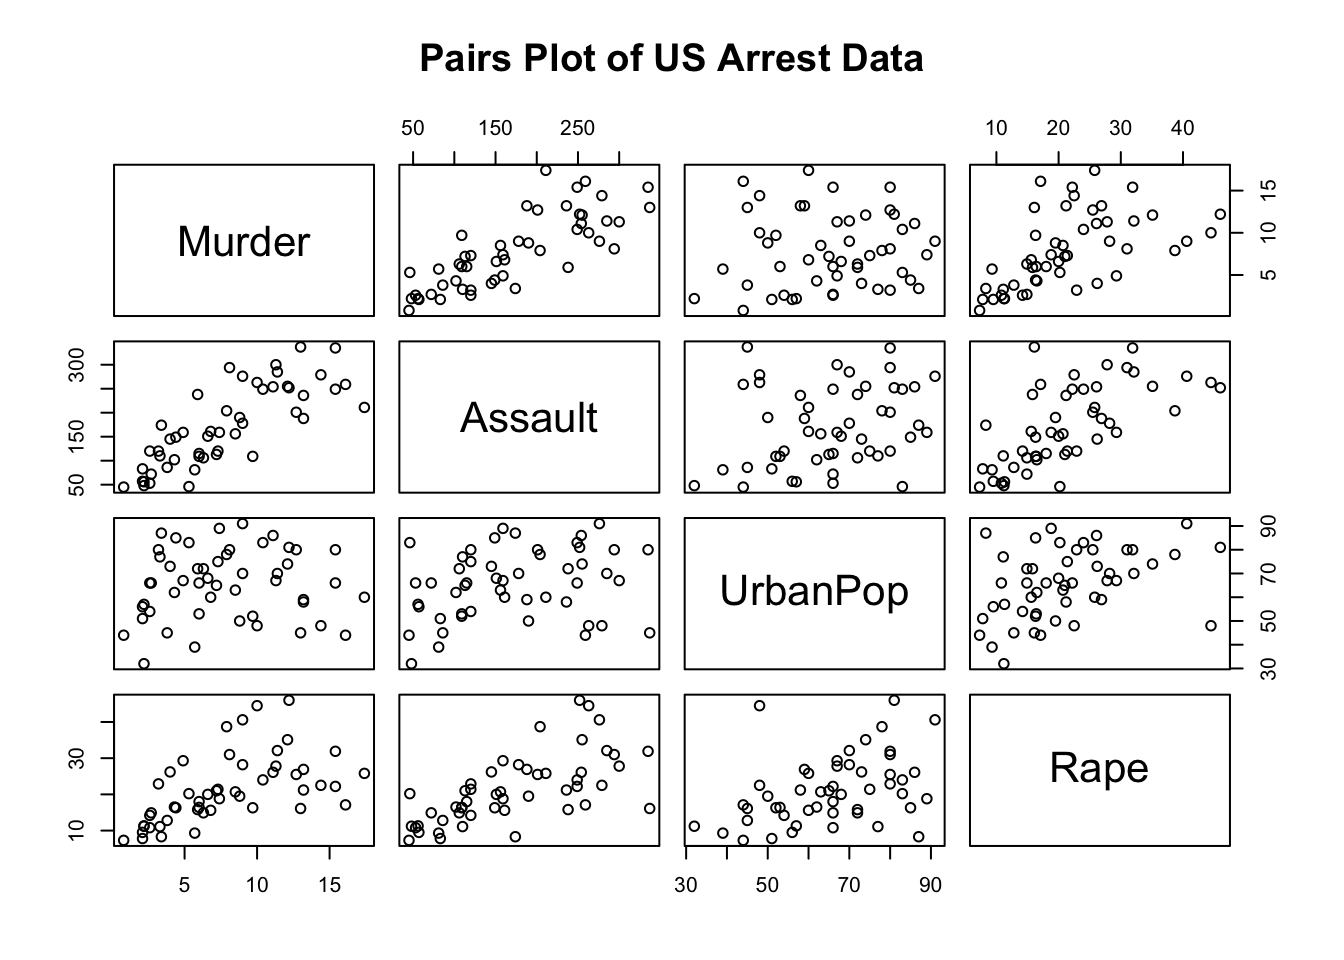
\includegraphics{RLabLab_files/figure-latex/unnamed-chunk-9-1.pdf}

\begin{Shaded}
\begin{Highlighting}[]
\FunctionTok{plot}\NormalTok{(USArrests}\SpecialCharTok{$}\NormalTok{Murder, USArrests}\SpecialCharTok{$}\NormalTok{Assault, }\AttributeTok{main =} \StringTok{"Murder vs Assault"}\NormalTok{, }\AttributeTok{xlab =} \StringTok{"Murder Rate"}\NormalTok{, }\AttributeTok{ylab =} \StringTok{"Assault Rate"}\NormalTok{)}
\end{Highlighting}
\end{Shaded}

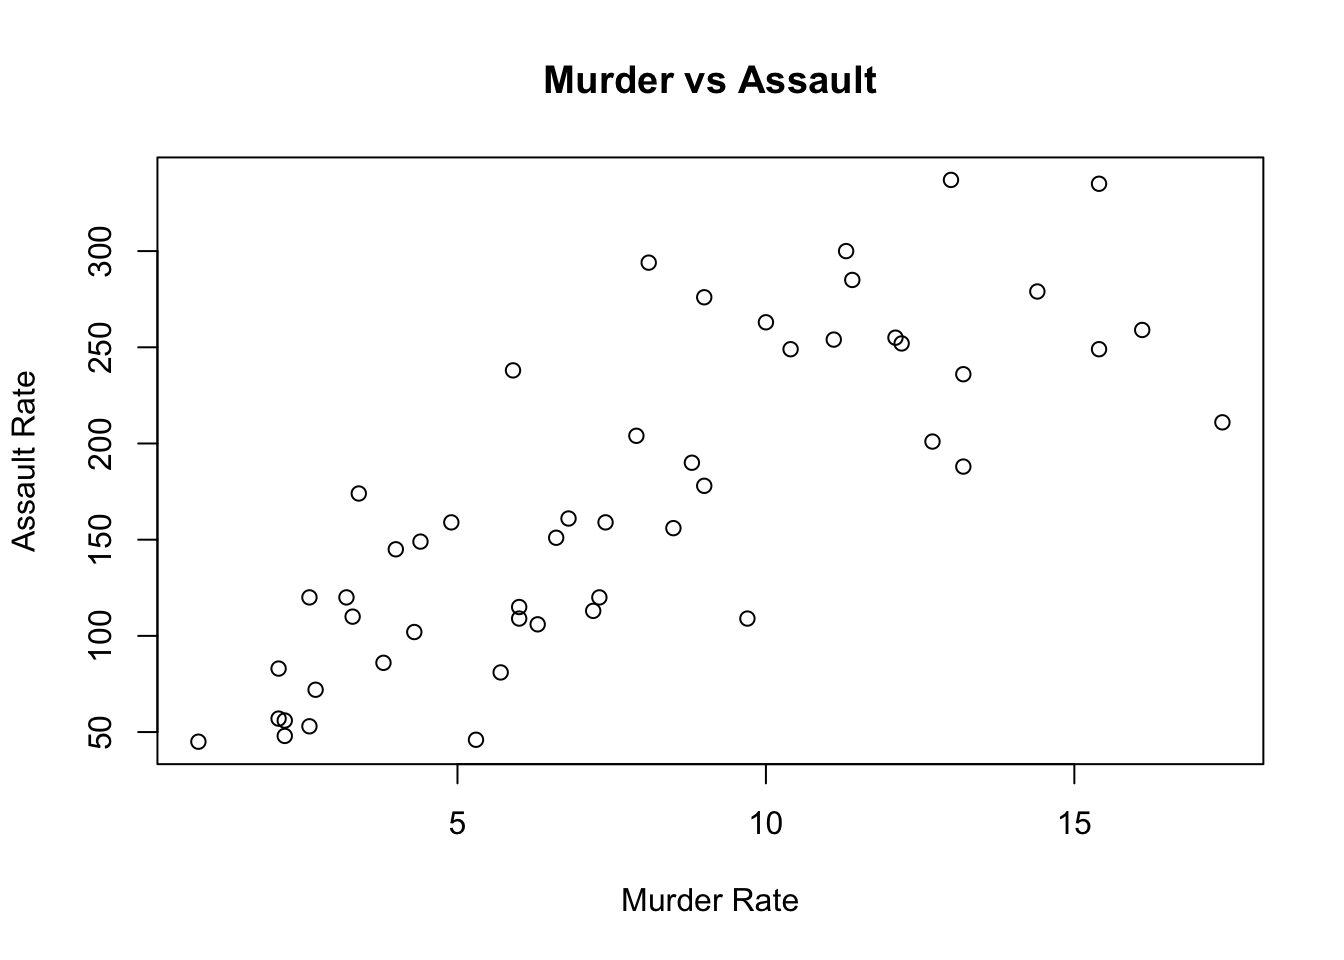
\includegraphics{RLabLab_files/figure-latex/unnamed-chunk-9-2.pdf}

Result: The pairs plot shows that murder and assault rates are
positively correlated, meaning states with more murders also have more
assaults. However, the urban population (UrbanPop) does not show a
strong relationship with any crime rates. The relationship between rape
and other crimes is weaker but still slightly positive. Overall, murder
and assault are more closely related, while urban population does not
appear to influence crime rates significantly.

=\textgreater{} Report a paragraph to summarize your findings from the
plot!

\begin{center}\rule{0.5\linewidth}{0.5pt}\end{center}

\subsubsection{Question 3}\label{question-3}

Download the housing data set from www.jaredlander.com and find out what
explains the housing prices in New York City.

Note: Check your working directory to make sure that you can download
the data into the data folder.

\begin{enumerate}
\def\labelenumi{\alph{enumi}.}
\tightlist
\item
  Create your own descriptive statistics and aggregation tables to
  summarize the data set and find any meaningful results between
  different variables in the data set.
\end{enumerate}

\begin{Shaded}
\begin{Highlighting}[]
\CommentTok{\# Head of the cleaned data set}

\NormalTok{housingData }\OtherTok{\textless{}{-}}\FunctionTok{read.csv}\NormalTok{(}\StringTok{"housing.csv"}\NormalTok{)}

\FunctionTok{head}\NormalTok{(housingData)}
\end{Highlighting}
\end{Shaded}

\begin{verbatim}
##   Neighborhood Building.Classification Total.Units Year.Built Gross.SqFt
## 1    FINANCIAL          R9-CONDOMINIUM          42       1920      36500
## 2    FINANCIAL          R4-CONDOMINIUM          78       1985     126420
## 3    FINANCIAL          RR-CONDOMINIUM         500         NA     554174
## 4    FINANCIAL          R4-CONDOMINIUM         282       1930     249076
## 5      TRIBECA          R4-CONDOMINIUM         239       1985     219495
## 6      TRIBECA          R4-CONDOMINIUM         133       1986     139719
##   Estimated.Gross.Income Gross.Income.per.SqFt Estimated.Expense
## 1                1332615                 36.51            342005
## 2                6633257                 52.47           1762295
## 3               17310000                 31.24           3543000
## 4               11776313                 47.28           2784670
## 5               10004582                 45.58           2783197
## 6                5127687                 36.70           1497788
##   Expense.per.SqFt Net.Operating.Income Full.Market.Value Market.Value.per.SqFt
## 1             9.37               990610           7300000                200.00
## 2            13.94              4870962          30690000                242.76
## 3             6.39             13767000          90970000                164.15
## 4            11.18              8991643          67556006                271.23
## 5            12.68              7221385          54320996                247.48
## 6            10.72              3629899          26737996                191.37
##        Boro
## 1 Manhattan
## 2 Manhattan
## 3 Manhattan
## 4 Manhattan
## 5 Manhattan
## 6 Manhattan
\end{verbatim}

\begin{Shaded}
\begin{Highlighting}[]
\CommentTok{\# Enter your code here!}
\FunctionTok{install.packages}\NormalTok{(}\StringTok{"dplyr"}\NormalTok{)  }
\end{Highlighting}
\end{Shaded}

\begin{verbatim}
## 
## The downloaded binary packages are in
##  /var/folders/6h/lg249dt14bq9ygh554ll961r0000gn/T//Rtmpc1liop/downloaded_packages
\end{verbatim}

\begin{Shaded}
\begin{Highlighting}[]
\FunctionTok{library}\NormalTok{(dplyr)}
\end{Highlighting}
\end{Shaded}

\begin{verbatim}
## 
## Attaching package: 'dplyr'
\end{verbatim}

\begin{verbatim}
## The following objects are masked from 'package:stats':
## 
##     filter, lag
\end{verbatim}

\begin{verbatim}
## The following objects are masked from 'package:base':
## 
##     intersect, setdiff, setequal, union
\end{verbatim}

\begin{Shaded}
\begin{Highlighting}[]
\NormalTok{agg\_table }\OtherTok{\textless{}{-}}\NormalTok{ housingData }\SpecialCharTok{\%\textgreater{}\%}
  \FunctionTok{group\_by}\NormalTok{(Boro) }\SpecialCharTok{\%\textgreater{}\%}
  \FunctionTok{summarise}\NormalTok{(}
    \AttributeTok{Avg\_Gross\_SqFt =} \FunctionTok{mean}\NormalTok{(Gross.SqFt, }\AttributeTok{na.rm =} \ConstantTok{TRUE}\NormalTok{),}
    \AttributeTok{Avg\_Income =} \FunctionTok{mean}\NormalTok{(Estimated.Gross.Income, }\AttributeTok{na.rm =} \ConstantTok{TRUE}\NormalTok{),}
    \AttributeTok{Avg\_Expense =} \FunctionTok{mean}\NormalTok{(Estimated.Expense, }\AttributeTok{na.rm =} \ConstantTok{TRUE}\NormalTok{),}
    \AttributeTok{Avg\_Net\_Operating\_Income =} \FunctionTok{mean}\NormalTok{(Net.Operating.Income, }\AttributeTok{na.rm =} \ConstantTok{TRUE}\NormalTok{),}
    \AttributeTok{Avg\_Market\_Value =} \FunctionTok{mean}\NormalTok{(Full.Market.Value, }\AttributeTok{na.rm =} \ConstantTok{TRUE}\NormalTok{)}
\NormalTok{  )}

\FunctionTok{print}\NormalTok{(agg\_table)}
\end{Highlighting}
\end{Shaded}

\begin{verbatim}
## # A tibble: 5 x 6
##   Boro          Avg_Gross_SqFt Avg_Income Avg_Expense Avg_Net_Operating_Income
##   <chr>                  <dbl>      <dbl>       <dbl>                    <dbl>
## 1 Bronx                172666.   2110718.    1137624.                  973094.
## 2 Brooklyn              37946.    736030.     314294.                  421736.
## 3 Manhattan            109186.   4185050.    1232606.                 2952444.
## 4 Queens                58610.   1056390.     437756.                  618634.
## 5 Staten Island         80781.   1066975.     516099.                  550876.
## # i 1 more variable: Avg_Market_Value <dbl>
\end{verbatim}

\begin{Shaded}
\begin{Highlighting}[]
\NormalTok{correlations }\OtherTok{\textless{}{-}} \FunctionTok{cor}\NormalTok{(housingData[, }\FunctionTok{c}\NormalTok{(}\StringTok{"Gross.SqFt"}\NormalTok{, }\StringTok{"Estimated.Gross.Income"}\NormalTok{, }\StringTok{"Estimated.Expense"}\NormalTok{, }
                                     \StringTok{"Net.Operating.Income"}\NormalTok{, }\StringTok{"Full.Market.Value"}\NormalTok{)], }\AttributeTok{use =} \StringTok{"complete.obs"}\NormalTok{)}
\FunctionTok{print}\NormalTok{(correlations)}
\end{Highlighting}
\end{Shaded}

\begin{verbatim}
##                        Gross.SqFt Estimated.Gross.Income Estimated.Expense
## Gross.SqFt              1.0000000              0.8560584         0.9433135
## Estimated.Gross.Income  0.8560584              1.0000000         0.9576951
## Estimated.Expense       0.9433135              0.9576951         1.0000000
## Net.Operating.Income    0.7945727              0.9918870         0.9133413
## Full.Market.Value       0.7747158              0.9829985         0.8982289
##                        Net.Operating.Income Full.Market.Value
## Gross.SqFt                        0.7945727         0.7747158
## Estimated.Gross.Income            0.9918870         0.9829985
## Estimated.Expense                 0.9133413         0.8982289
## Net.Operating.Income              1.0000000         0.9940990
## Full.Market.Value                 0.9940990         1.0000000
\end{verbatim}

\begin{enumerate}
\def\labelenumi{\alph{enumi}.}
\setcounter{enumi}{1}
\tightlist
\item
  Create multiple plots to demonstrates the correlations between
  different variables. Remember to label all axes and give title to each
  graph.
\end{enumerate}

\begin{Shaded}
\begin{Highlighting}[]
\CommentTok{\# Enter your code here!}
\FunctionTok{install.packages}\NormalTok{(}\StringTok{"ggplot2"}\NormalTok{)}
\end{Highlighting}
\end{Shaded}

\begin{verbatim}
## 
## The downloaded binary packages are in
##  /var/folders/6h/lg249dt14bq9ygh554ll961r0000gn/T//Rtmpc1liop/downloaded_packages
\end{verbatim}

\begin{Shaded}
\begin{Highlighting}[]
\FunctionTok{library}\NormalTok{(ggplot2)}
\FunctionTok{ggplot}\NormalTok{(housingData, }\FunctionTok{aes}\NormalTok{(}\AttributeTok{x =}\NormalTok{ Gross.SqFt, }\AttributeTok{y =}\NormalTok{ Full.Market.Value)) }\SpecialCharTok{+}
  \FunctionTok{geom\_point}\NormalTok{() }\SpecialCharTok{+}
  \FunctionTok{labs}\NormalTok{(}\AttributeTok{title =} \StringTok{"Gross Square Footage vs Full Market Value"}\NormalTok{,}
       \AttributeTok{x =} \StringTok{"Gross Square Footage"}\NormalTok{,}
       \AttributeTok{y =} \StringTok{"Full Market Value"}\NormalTok{)}
\end{Highlighting}
\end{Shaded}

\includegraphics{RLabLab_files/figure-latex/unnamed-chunk-12-1.pdf}

\begin{Shaded}
\begin{Highlighting}[]
\FunctionTok{ggplot}\NormalTok{(housingData, }\FunctionTok{aes}\NormalTok{(}\AttributeTok{x =}\NormalTok{ Estimated.Gross.Income, }\AttributeTok{y =}\NormalTok{ Full.Market.Value)) }\SpecialCharTok{+}
  \FunctionTok{geom\_point}\NormalTok{() }\SpecialCharTok{+}
  \FunctionTok{labs}\NormalTok{(}\AttributeTok{title =} \StringTok{"Estimated Gross Income vs Full Market Value"}\NormalTok{,}
       \AttributeTok{x =} \StringTok{"Estimated Gross Income"}\NormalTok{,}
       \AttributeTok{y =} \StringTok{"Full Market Value"}\NormalTok{)}
\end{Highlighting}
\end{Shaded}

\includegraphics{RLabLab_files/figure-latex/unnamed-chunk-12-2.pdf}

\begin{Shaded}
\begin{Highlighting}[]
\FunctionTok{ggplot}\NormalTok{(housingData, }\FunctionTok{aes}\NormalTok{(}\AttributeTok{x =}\NormalTok{ Estimated.Expense, }\AttributeTok{y =}\NormalTok{ Net.Operating.Income)) }\SpecialCharTok{+}
  \FunctionTok{geom\_point}\NormalTok{() }\SpecialCharTok{+}
  \FunctionTok{labs}\NormalTok{(}\AttributeTok{title =} \StringTok{"Estimated Expense vs Net Operating Income"}\NormalTok{,}
       \AttributeTok{x =} \StringTok{"Estimated Expense"}\NormalTok{,}
       \AttributeTok{y =} \StringTok{"Net Operating Income"}\NormalTok{)}
\end{Highlighting}
\end{Shaded}

\includegraphics{RLabLab_files/figure-latex/unnamed-chunk-12-3.pdf}

\begin{enumerate}
\def\labelenumi{\alph{enumi}.}
\setcounter{enumi}{2}
\tightlist
\item
  Write a summary about your findings from this exercise.
\end{enumerate}

The plots show a clear positive relationship between the size of a
property and its market value---larger properties tend to be worth more.
Properties that earn more income also have a higher market value.
Lastly, while properties with higher expenses also tend to generate more
income, the relationship is not as strong as with the othe

=\textgreater{} Enter your answer here!

This analysis shows that larger properties and those in Manhattan tend
to have the highest market values and income. There is a clear positive
relationship between property size, income generation, and market value.
Higher expenses can reduce net income, but the effect varies across
properties. Overall, location and size are key factors driving property
value.

\end{document}
